\documentclass[12pt,a4paper,brazilian, fleqn]{article}

\usepackage{babel}
\usepackage[utf8]{inputenc}
\usepackage[T1]{fontenc}
\usepackage{lmodern}

\usepackage{amssymb,amsfonts,amsmath}

\usepackage{tikz}
\usetikzlibrary{calc,intersections}

%https://tex.stackexchange.com/a/100406
%29.7 cm - 1cm - 1cm - 144.90/28.4 cm = 22.60 cm
\usepackage[a4paper, totalheight=22.60cm,includeheadfoot,left=1.5cm, right=1.0cm, top=1cm]{geometry}
\setlength{\headheight}{144.90pt}

\setkeys{Gin}{keepaspectratio}

\newcommand{\cabeca}{
    \begin{tikzpicture}
        \node(Logo) {
\includegraphics[width=2.5cm]{logo.png}};
        % \node(Logo) {
\includegraphics[width=4.1cm]{logo.png}};

        \node(Local) at (Logo.north east) [anchor=north west, yshift=-0.25cm,
            align=center, execute at begin node=\setlength{\baselineskip}{3ex}]
            {
                \huge{\textbf{Universidade Federal do Amazonas}} \\
                \large{\textbf{Instituto de Ciências Exatas e Tecnologia}} \\
                \large{\textbf{\Description}}
            };

        \node(Ident) at (Local.south west) [anchor=north west, yshift=-0.25cm,
            align=left, execute at begin node=\setlength{\baselineskip}{2em}]
            {
                Professor: {\fontfamily{augie}\selectfont \Professor} \\
                Aluno(s):
            };
        % \draw [thick] (Logo.south west) -- ($(Logo.south west -| Local.south east)$);
        % \draw [red] (Logo.north west) rectangle (Logo.south east);
        % \draw [blue] (Local.north west) rectangle (Local.south east);
        % \draw [green] (Ident.north west) rectangle (Ident.south east);
    \end{tikzpicture}
}

\usepackage{fancyhdr}
\fancyhead{}
\fancyfoot{}
\fancyhead[c]{\cabeca}
\fancyfoot[r]{\fontfamily{augie}\selectfont Boa sorte!}

\pagestyle{fancy}
\renewcommand{\headrulewidth}{0pt}
\renewcommand{\footrulewidth}{0pt}

\newcommand{\ratio}[1]{(#1\% da nota)}
%-----------------------------------CUT HERE-----------------------------------

\def\Description{Fenômenos de Transporte -- Prova 1}
\def\Professor{Rodrigo de Farias Gomes}

\usepackage{siunitx}
\sisetup{locale = FR}

\usepackage{tcolorbox}
\tcbset{boxrule=0pt, top=0pt, bottom=0pt}

\DeclareMathOperator{\sen}{sen}
\DeclareMathOperator{\tg}{tg}
\usepackage{enumitem}
\usepackage{calc}

\begin{document}

\begin{tcolorbox}[colback=black!10, colframe=black!50, title=Observações]
    \begin{itemize}
        \item Todas as páginas com resposta devem ter o nome e matrícula do
            aluno escritos com caneta no início (cabeçalho) ou no final
            (rodapé). Páginas que não obedeçam a esse critério não serão usadas
            na avaliação
    \end{itemize}
\end{tcolorbox}

\vspace{2em}

\begin{enumerate}
    \item \ratio{35} O eixo da figura abaixo, ao girar, provoca a rotação do tambor.
        Este enrola a corda, que levanta um peso de 15 N com uma velocidade constante
        de \SI{0.5}{m/s}. O fluido existente entre o eixo e o tambor tem
        \(\mu = \SI{0.1}{N.s/m^2}\) e apresenta um diagrama linear de velocidades.
        Pede-se:
        \begin{enumerate}
            \item a rotação do eixo em rpm;
            \item o momento provocado pelo fluido contra a rotação do eixo.
        \end{enumerate}
        \textit{Dados}: \(R_1 = \SI{10}{cm}\); \(R_2 = \SI{10.1}{cm}\);
        \(R_3 = \SI{20}{cm}\); \(\omega = 2 n \pi\).

        \begin{center}
            \includegraphics[width=\textwidth-30pt]{figura_para_prova.pdf}
        \end{center}

        \newpage

    \item \ratio{30} A figura abaixo mostra um esquema de um recipiente pressurizado
        contendo água, com um manômetro de tubo em ''U'' conectado na altura do 
        ponto \(A\). Determine a pressão existente no ponto \(A\) como uma função
        de \(\rho_A\), \(h_1\), \(h_2\), \(\rho_M\) e \(p_\text{atm}\)

        \begin{center}
            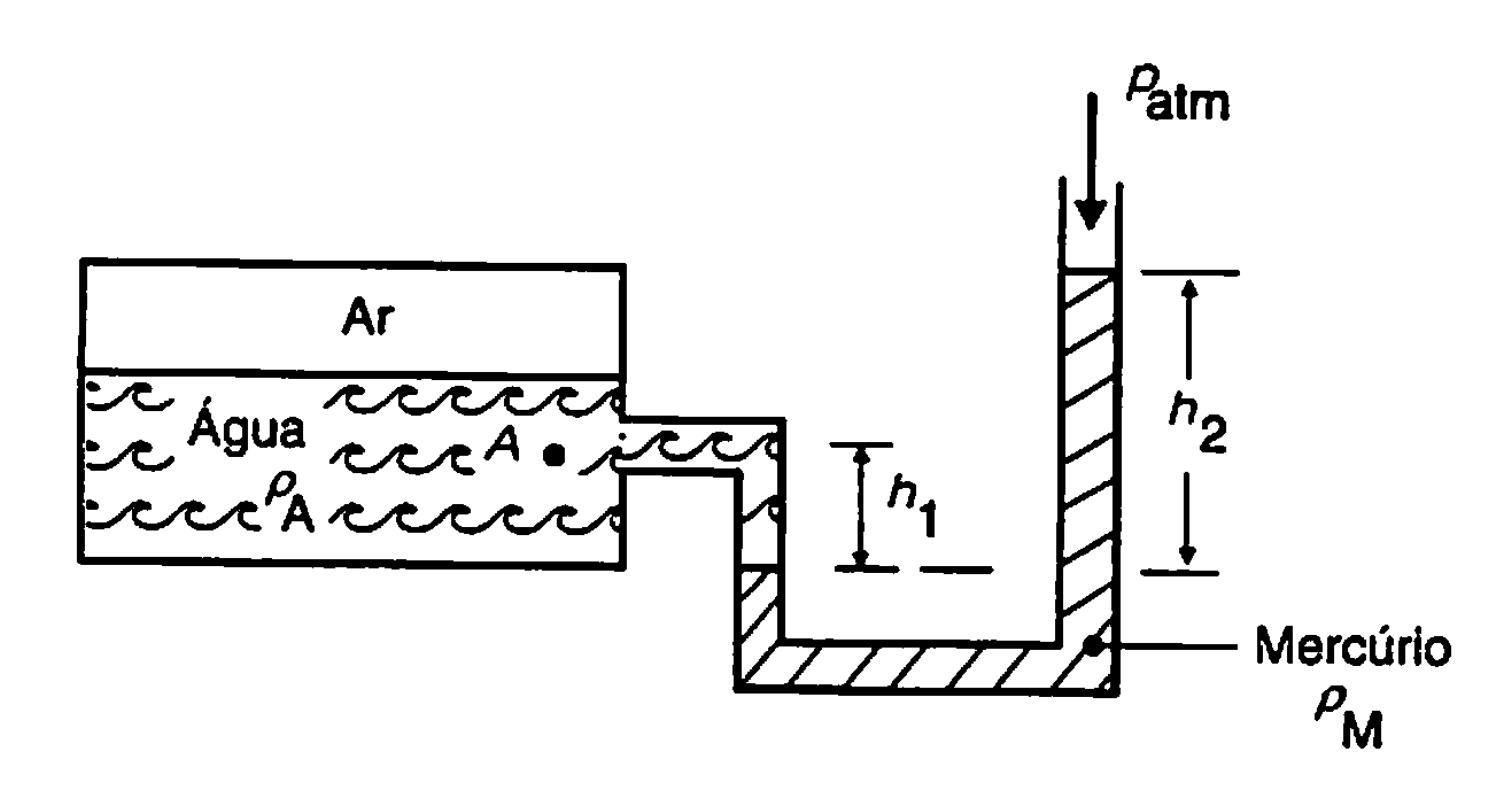
\includegraphics[width=0.5\textwidth]{Captura de tela 2025-06-03 133507.png}
        \end{center}

    \item \ratio{35} A figura abaixo mostra um esquema de uma janela triangular de 
        base \(B=\SI{1.5}{m}\) e altura \(H=\SI{1.5}{m}\), localizada na parede 
        vertical de um tanque com água e aberto para a atmosfera. Determine a
        força resultante exercida pela água sobre a janela e a profundidade de seu ponto 
        de aplicação.

        \begin{center}
            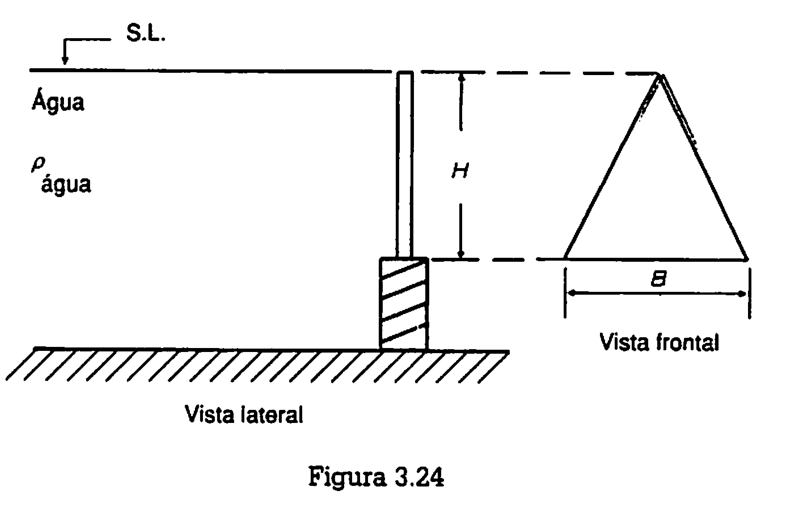
\includegraphics[width=0.5\textwidth]{Captura de tela 2025-06-03 134107.png}
        \end{center}
\end{enumerate}

Informações \textit{possivelmente} úteis:
\begin{itemize}
    \item Área de um triângulo de base \(b\) e altura \(L\): \(A=bL/2\)
    \item Segundo momento da área de um triângulo de base \(b\) e altura \(L\) em relação ao eixo que passa pelo centróide:
        \(I_{cc} = bL^3/36\)
    \item Componente vertical da posição do centróide de um triângulo
        de base \(b\) e altura \(L\), considerando a origem na base: \(y=L/3\)
\end{itemize}

\end{document}
